% IEEEtran 在类初始化时使用传统字体编码；正文随后由 fontspec 切换至 Unicode 字体。
\RequirePackage[T1]{fontenc}
\documentclass[journal,10pt,a4paper]{IEEEtran}

% 中文使用 TeX Live / Overleaf 随附的 Fandol 字体，保留 IEEEtran 标题与双栏格式。
\usepackage[UTF8,scheme=plain,fontset=none]{ctex}
\setmainfont{texgyretermes-regular.otf}[
  BoldFont=texgyretermes-bold.otf,
  ItalicFont=texgyretermes-italic.otf,
  BoldItalicFont=texgyretermes-bolditalic.otf
]
\setsansfont{texgyreheros-regular.otf}[
  BoldFont=texgyreheros-bold.otf,
  ItalicFont=texgyreheros-italic.otf,
  BoldItalicFont=texgyreheros-bolditalic.otf
]
% 为 IEEEtran 使用的粗斜体和小型大写样式明确指定中文对应字形。
\setCJKmainfont{FandolSong-Regular.otf}[
  BoldFont=FandolSong-Bold.otf,
  ItalicFont=FandolKai-Regular.otf,
  BoldItalicFont=FandolHei-Bold.otf,
  SmallCapsFont=FandolSong-Regular.otf
]
\setCJKsansfont{FandolHei-Regular.otf}[BoldFont=FandolHei-Bold.otf]
\setCJKmonofont{FandolFang-Regular.otf}
\usepackage{graphicx}
\usepackage{booktabs}
\usepackage{tabularx}
\usepackage{array}
% 允许跨栏图表在页顶或页底排版，并在所属章节收束。
\usepackage{stfloats}
\usepackage[section]{placeins}
\usepackage[hidelinks,unicode]{hyperref}

\renewcommand{\abstractname}{摘要}
\renewcommand{\figurename}{Figure}
\renewcommand{\tablename}{Table}
\renewcommand{\thetable}{\arabic{table}}
\graphicspath{{figures/}}
\newcolumntype{Y}{>{\raggedright\arraybackslash}X}
% 仅为窄栏中的长英文词提供适量断行余量。
\setlength{\emergencystretch}{1em}
\setcounter{secnumdepth}{0}
\setcounter{dbltopnumber}{1}
\setcounter{dblbotnumber}{1}
\pagestyle{plain}
\raggedbottom

\title{面向真实物理无线链路的联邦学习实验平台设计与性能评估}
% 源稿没有作者及单位信息，确认后在此填写 \author{...}。
\author{}

\begin{document}
\maketitle
\thispagestyle{plain}

\begin{abstract}
[待定稿后撰写]
\end{abstract}

\section{引言}
\label{sec:1}

联邦学习允许多台边缘设备在保留本地数据的前提下协同训练全局模型。当训练节点延伸至移动终端、车载计算平台或各类传感器时，中心服务端分发全局模型参数，以及各设备回传本地计算得到的模型更新，均落在真实的物理无线链路之上。每轮通信耗费的时间，不仅取决于模型文件的大小，也直接受制于当时当地的无线传输条件。主流的联邦学习编排框架通常面向通用网络环境设计，将底层通信逻辑封装在标准套接字与传输层连接之后。对分布式算法开发而言，这种分层抽象非常省心。但若研究重点恰恰是无线环境本身，问题就会暴露出来。常规网络接口只暴露数据收发与连接状态，研究人员既无法主动设定底层无线参数，也难以在相同实验条件下，把具体的无线配置与整轮训练耗时联系起来系统比较。

在真实物理信道中，无线传输的表现取决于多项具体的收发设置。其中，调制编码方案（MCS）决定单帧的调制阶数与编码率，信道带宽决定频带宽度，符号保护间隔（GI）用来抵抗多径反射引起的时延扩展，前向纠错（FEC）在数据包层面添加校验冗余以抵御突发丢帧，发射功率则决定天线端的发射强度。常规商用 Wi-Fi 网卡为了维持连接稳定，往往由固件在后台自动调节传输速率。这种自适应机制会根据瞬时信道质量频繁升降调制阶数，导致每次发送的物理参数自行漂移。对受控实验而言，这就带来了麻烦。实验人员既无法锁定一组指定的无线参数开展严谨测试，也难以在不同轮次间重现完全相同的传输设置。一旦某个客户端回传滞后，或者整轮耗时大幅拉长，研究人员仅凭应用层暴露的耗时数字，很难弄清通信表现究竟与哪些无线参数直接相关。

针对这一局限，本文提出基于消费级 802.11 硬件，把联邦学习中的真实无线链路转变为可主动配置条件且可记录接收信息的实验对象。平台的设计目标，是支持研究人员在固定模型结构、数据集与计算条件的前提下，主动设定不同的无线参数组合，进而在完整训练流程中定量对比模型分发吞吐、客户端更新提交进展以及整轮耗时。在技术途径上，平台借助消费级网卡的监听模式（monitor 模式）与原始帧注入绕过商用固件的控制逻辑。网卡开启监听模式后脱离常规接入点的关联流程，直接捕获空中实际到达的无线帧，并记录随帧附带的物理层元数据，例如实际接收到的调制编码方案索引与信号强度。在模型下行分发时由客户端记录接收信息，在上行更新回传时由服务端记录。原始帧注入则赋予发送端绕过系统默认协商机制的能力，直接按照实验预设的参数构造并送出 802.11 物理帧。各项无线条件的配置分别落在不同的系统层次。工作信道、带宽与发射功率通过驱动与内核接口直接下发给射频芯片。调制编码方案与保护间隔由发送端在构造单帧时写入发射描述信息，由物理层逐帧采纳。前向纠错则运行在链路控制层，通过通用处理器对数据分组计算块级校验冗余，与底层射频配置分属不同层级。

消费级 802.11 硬件为这类受控实验带来了切实的设备可获得性。市售的双频 USB 无线网卡单价在百元级，依托免许可频段工作，不需要申请专门的无线电执照，研究团队很容易备齐多节点实验所需的外设。不过，设备易得并不等同于系统开箱即用。这套方案依赖特定网卡芯片与开源驱动补丁来支持监听和帧注入，实验人员依然需要在多台边缘节点上逐一配置系统环境、编译专用驱动并联调收发控制逻辑。此外，实验参数可配置，并不代表真实世界的复杂电磁环境能够被完全掌控或精确复制。通信对端记录的帧级元数据，也无法替代专用射频仪表的连续信道估计。平台的作用，在于为研究人员提供一套低成本且可行的实验工具，在真实硬件上把物理无线配置与端到端联邦学习流程结合起来，支持有依据的对比测试与通信特征分析。

\section{无线实验平台的选择与比较}
\label{sec:2}

系统比较不同无线配置对端到端训练流程的影响，对实验平台的收发能力提出了明确的技术诉求。一方面，参数与发送行为必须可控，从而支持研究人员主动构造差异化的实验条件，在保持模型结构、训练数据和本地计算负载完全一致的前提下，观察通信耗时与轮次推进的变化。另一方面，平台应当支持高效的一对多模型分发。联邦学习每轮下行都需要将完全相同的全局模型推送到全体参与客户端，广播传输可以有效避免单播方式带来的重复发送开销。尽管单播同样能够完成真实的无线联邦学习实验，但随着客户端数量增加，广播在减少网络占用方面的优势会更加明显。

围绕上述实验目标，研究者通常有几种不同的实验平台搭建路径，各自存在不同的工程特征与使用条件（见 Table~\ref{tab:1}）。常见的做法是采用消费级 Wi-Fi 的常规联网方式。商用无线网卡与接入点容易获得且价格低廉，网络配置相当成熟。但常规网络协议栈把物理层收发细节封装在固件与驱动之内，固件内置的速率自适应机制会在后台频繁升降调制阶数，导致实验人员很难锁定一组预设的无线参数进行受控对比。同时，标准接入点往往将广播帧限制在较低的基本速率集，分发数十兆字节的模型文件需要消耗较多时间。第二种途径是基于低功耗蓝牙构建测试环境。低功耗蓝牙硬件小巧、能耗极低且单价只有数十元，非常适合大规模低功耗节点的互联。但在协议标准规范下，其物理层数据速率通常在 1 至 2 Mbps 之间，单包有效载荷也较小，面对数十兆字节的深度学习模型文件时分发耗时漫长，更适合承载参数量较小的轻量级模型或局部更新。若追求更高的物理层灵活性，研究者往往转向软件定义无线电。通过软件定义无线电平台，研究人员可以直接在基带层面灵活定制调制格式、纠错编码与射频参数，具备极高的可编程性。然而，这类硬件的采购成本显著偏高，单节点设备从数千元到数万元不等。更为关键的是，研究团队需要自行实现或深度移植完整的介质访问控制与高层传输协议栈，系统维护工作繁重，且在部分频段发射无线信号时还需要取得专门的无线电管理频谱许可。

% 原稿标记保留：**[Table 1 占位 无线实验平台搭建方案对比矩阵]**

% 原稿题注保留：> Table 1 按关键无线参数可控性、广播分发能力、硬件成本与部署维护条件四个维度，对比四种无线实验搭建方案的实现特征与使用条件。

\begin{table*}[tb]
\caption{无线实验平台搭建方案对比。}
\label{tab:1}
\centering
\small
\renewcommand{\arraystretch}{1.25}
\setlength{\tabcolsep}{5pt}
\begin{tabularx}{\textwidth}{@{}>{\raggedright\arraybackslash}p{0.12\textwidth}YYYY@{}}
\toprule
\textbf{评估维度} & \textbf{采用消费级 Wi-Fi 常规联网方式的方案} & \textbf{基于低功耗蓝牙的方案} & \textbf{基于软件定义无线电的定制方案} & \textbf{本文平台（WFB-FL）} \\
\midrule
\textbf{关键无线参数可控性} & 受固件自适应调节与驱动封装限制，通常难以在运行中锁定发送参数 & 参数主要由协议栈固化配置管理，物理层可调范围较窄 & 支持基带与射频参数的灵活软件定制 & 支持显式指定信道、带宽、MCS、保护间隔、FEC 与发射功率 \\
\textbf{广播分发能力} & 通常受限于接入点协商的基本速率集，亦可采用单播替代广播 & 受协议标准速率（1 至 2 Mbps）约束，分发大体积模型文件耗时较长 & 具备物理广播能力，但需自行实现可靠分发与重传协议栈 & 支持以高阶速率发送广播帧，由文件分发协议处理可靠交付 \\
\textbf{硬件成本} & 较低（单节点百元级商用网卡或路由设备） & 低（单节点数十元级射频模块） & 较高（单节点数千元至数万元不等） & 较低（单节点百元级消费级 USB 网卡） \\
\textbf{部署与维护条件} & 常规网络配置成熟，接入点部署方便 & 拓扑配置简单，管理开销小 & 需基带软硬件联合调试，在受保护频段需无线电管理许可 & 工作于免许可频段，需编译补丁驱动并调试收发协同逻辑 \\
\bottomrule
\end{tabularx}
\end{table*}

面向本文受控对比的实验目标，WFB-FL 将消费级 802.11 硬件、可设置的收发参数与面向模型分发的广播传输组合在同一方案中。平台依托双频 USB 无线网卡，利用开源驱动补丁开放监听模式（monitor 模式）与原始帧注入能力。在免许可频段上，发送端绕过标准连接协商，直接构造包含预设信道、带宽、MCS、保护间隔、FEC 冗余度与发射功率的物理帧，并以高阶速率向多客户端广播模型文件；通信对端则捕获空中实际到达的无线帧并记录元数据。这种机制为受控实验提供了主动调整物理参数与观察实际通信表现的途径，但也对应着具体的部署与维护代价。这套系统并非开箱即用。研究人员需要选用支持注入模式的特定芯片网卡，在各边缘节点上独立编译专用驱动补丁，并手动配置免许可频段的工作模式与节点间的调度时序。百元级的消费级硬件提供了切实的设备可获得性，而收发控制与多节点防碰撞则需要完全交由软件逻辑独立承担。

\section{WFB-FL 体系架构与端到端运作机制}
\label{sec:3}

为满足受控实验的收发要求，平台首先必须打通可控的无线收发能力，支持显式调节关键无线参数，并突破常规 Wi-Fi 对广播速率的限制。常规 Wi-Fi 很难做到这一点。商用固件全权接管物理层，在后台自行升降速率，并将广播帧锁死在低速的基本速率集。平台利用消费级网卡的 monitor 模式接收与原始帧注入绕过这一限制。开启 monitor 模式后，网卡脱离常规接入点的关联流程。通信对端直接捕获空中实际到达的无线帧，并记录随帧附带的 Radiotap 元数据，包括时间戳、工作频率、调制编码方案（MCS）索引与信号强度。原始帧注入则赋予发送端自主构造物理帧的能力。发送端越过操作系统内核的速率协商逻辑，把按指定参数组装的 802.11 帧直接送入无线信道。高阶物理速率的广播分发由此成为可能。

在此收发基础上，平台支持对六项关键无线参数实施显式设定，并依据不同的系统层次采用对应的配置途径。工作信道与频段、信道带宽以及发射功率，由网卡驱动与操作系统内核接口直接下发给射频芯片。决定单帧调制阶数与编码率的 MCS，以及用于抵御多径时延扩展的符号级保护间隔（GI），由发送端在构造原始帧时写入发射元数据，供物理层逐帧应用。用于抵御空口误码与突发丢帧的前向纠错（FEC），属于链路控制层对数据分组的冗余编码处理，由发送端为一组数据包附加密集校验块，与物理层编码配置处于不同层次。通信对端捕获到的物理帧与元数据，在下行由客户端记录，在上行由服务端记录，为后续实验提供直接的物理层核验依据。常规 802.11 广播机制本身缺乏逐接收端的硬件确认，而平台在虚拟网络接口之上依然复用成熟的网络协议。平台的核心任务是利用这些底层收发能力，为上层联邦学习构建可靠的一对多模型分发与有序的更新回传机制。

系统自上而下划分为五层（见 Fig.~\ref{fig:1}），各层职责边界分明。联邦学习算法层负责全局模型的训练评估与聚合逻辑。联邦学习运行层维护严格同步的训练轮次，编排模型发布、模型等待、更新提交与更新收齐。传输适配层承接模型与更新的文件交换需求，向下将其映射到具体传输协议，其中下行采用一对多文件分发协议 UFTP，上行采用 HTTP PUT 配合底层 TCP 传输。链路控制层以 TUN 虚拟网卡作为网络边界，管理发送许可、调度控制消息、出站发送队列与入站重组缓冲。无线收发层驱动无线网卡执行原始帧注入与 monitor 模式接收。调用自顶向下发起，完成结果逐层向上返回。TUN 虚拟网络接口承接上层普通数据流量，链路控制帧则由独立的控制通道直接传输，不经过 TUN 接口。

% 原稿标记保留：**[Figure 1 占位 WFB-FL 五层架构与简化端到端流程图]**

% 原稿题注保留：> Figure 1 展示服务端与多个客户端的五层职责划分、TUN 边界，以及模型下行、本地训练、更新上行与聚合的简化流程，并标明传输适配层在下行采用一对多文件分发协议 UFTP、在上行采用 HTTP PUT 与 TCP。

\begin{figure*}[tb]
\centering
% 裁去图稿上下的纯白外边距，保留所有图内元素；PDF 文件本身不变。
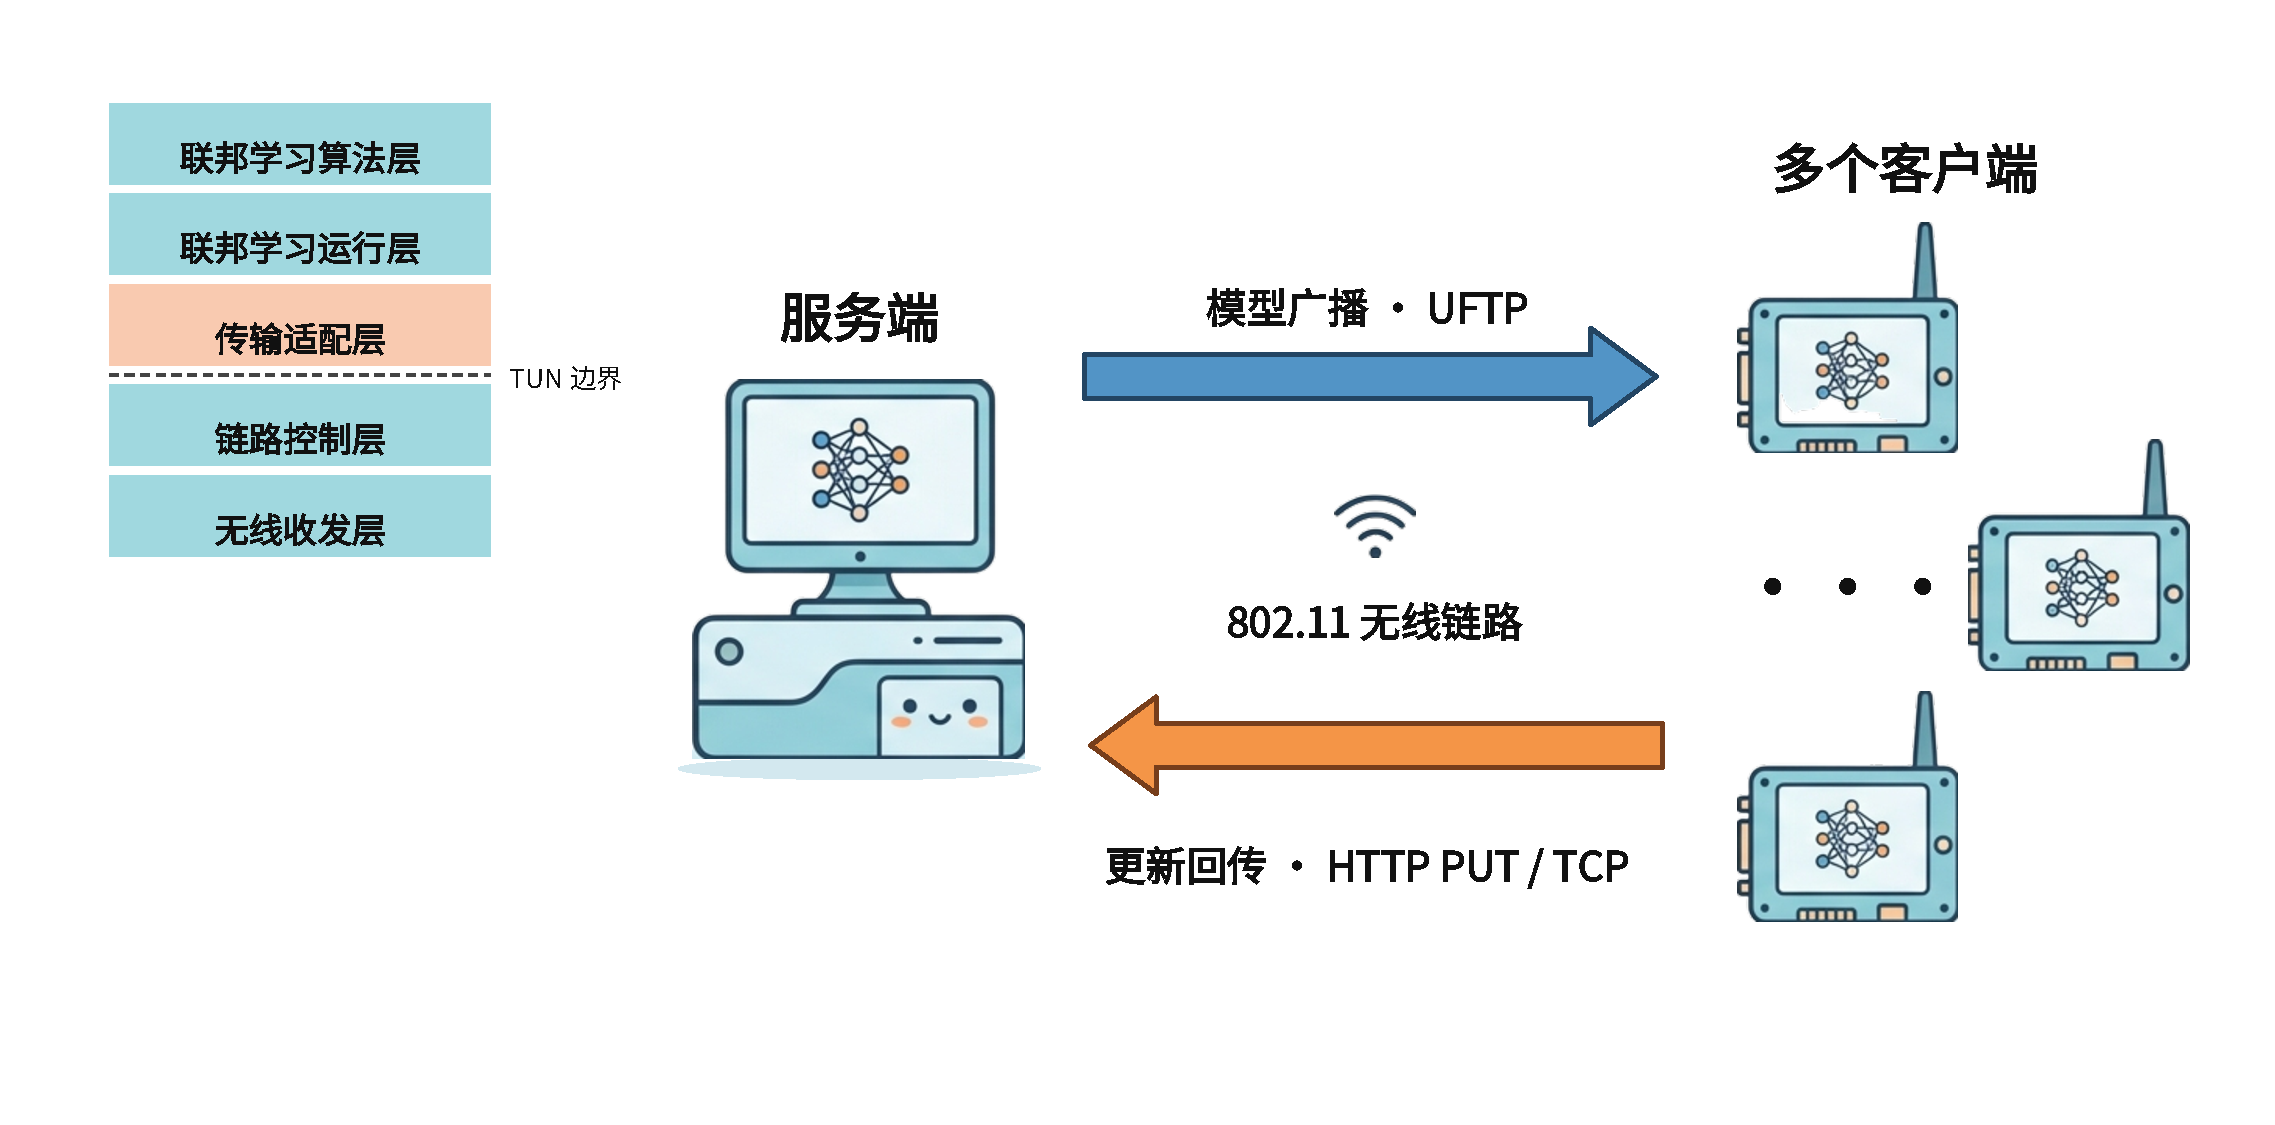
\includegraphics[width=\textwidth,trim=0 80bp 0 32bp,clip]{figure1.pdf}
\caption{WFB-FL 五层架构与简化端到端流程。}
\label{fig:1}
\end{figure*}

一轮联邦学习训练由服务端发起。算法层准备好全局模型，运行层冻结本轮参与训练的客户端集合并生成交付清单，交由传输适配层启动模型分发。下行传输选择一对多文件分发协议 UFTP。同一份全局模型要送到全体客户端手中，面对典型的一对多单向流量，直接复用成熟协议在分块、缺块反馈与选择性补发上的现成能力，可以省去重复实现复杂的可靠传输逻辑。高阶物理速率的无线广播由底层的原始帧注入直接提供，UFTP 则专注于在此广播承载之上保障文件交付的可靠性。广播帧在无线信道传输时可能因衰落或偶发干扰发生丢包，系统通过两道防线逐级恢复。第一道防线由链路控制层的前向纠错承担。发送端在分组层面附加纠错冗余块，客户端在接收到部分丢帧的情况下，只要成功捕获的分组数量达到恢复门限，即可在本地直接重构原始数据块。超出前向纠错恢复能力的个别缺块由第二道防线处理。客户端记录缺失数据块的编号并在反向反馈机会中告知服务端，服务端接收反馈后重新广播补发对应的数据块。

客户端回传缺块信息与完成状态时，多个客户端共享同一无线信道。多节点同时回传，信号必然在空中相互重叠与干扰。解决办法是发送权轮转（见 Fig.~\ref{fig:2}）。服务端定期暂停主广播，拿出当前活跃队列的快照，按顺序轮流给客户端发许可。许可对应一个固定时长的限时发送窗口。拿到窗口的客户端才能发数据，时间一到立刻停手。前后两个窗口之间还要留出固定的窗口切换间隔，留出足够的物理时间间隙，防止前后两台设备的无线信号发生交叠。发送权轮转机制旨在协调平台内部受管客户端的发送时机，有效降低彼此之间发生发送冲突与信号碰撞的可能。该机制并不改变开放无线环境的物理特性，无法阻止未受管外部设备的射频干扰，也不声称信道在物理层面上始终由单一节点独占。

% 原稿标记保留：**[Figure 2 占位 发送权轮转机制图]**

% 原稿题注保留：> Figure 2 解释限时发送机会在节点间的轮换过程、窗口到期停发特征以及相邻发送机会之间的窗口切换间隔。

\begin{figure*}[b]
\centering
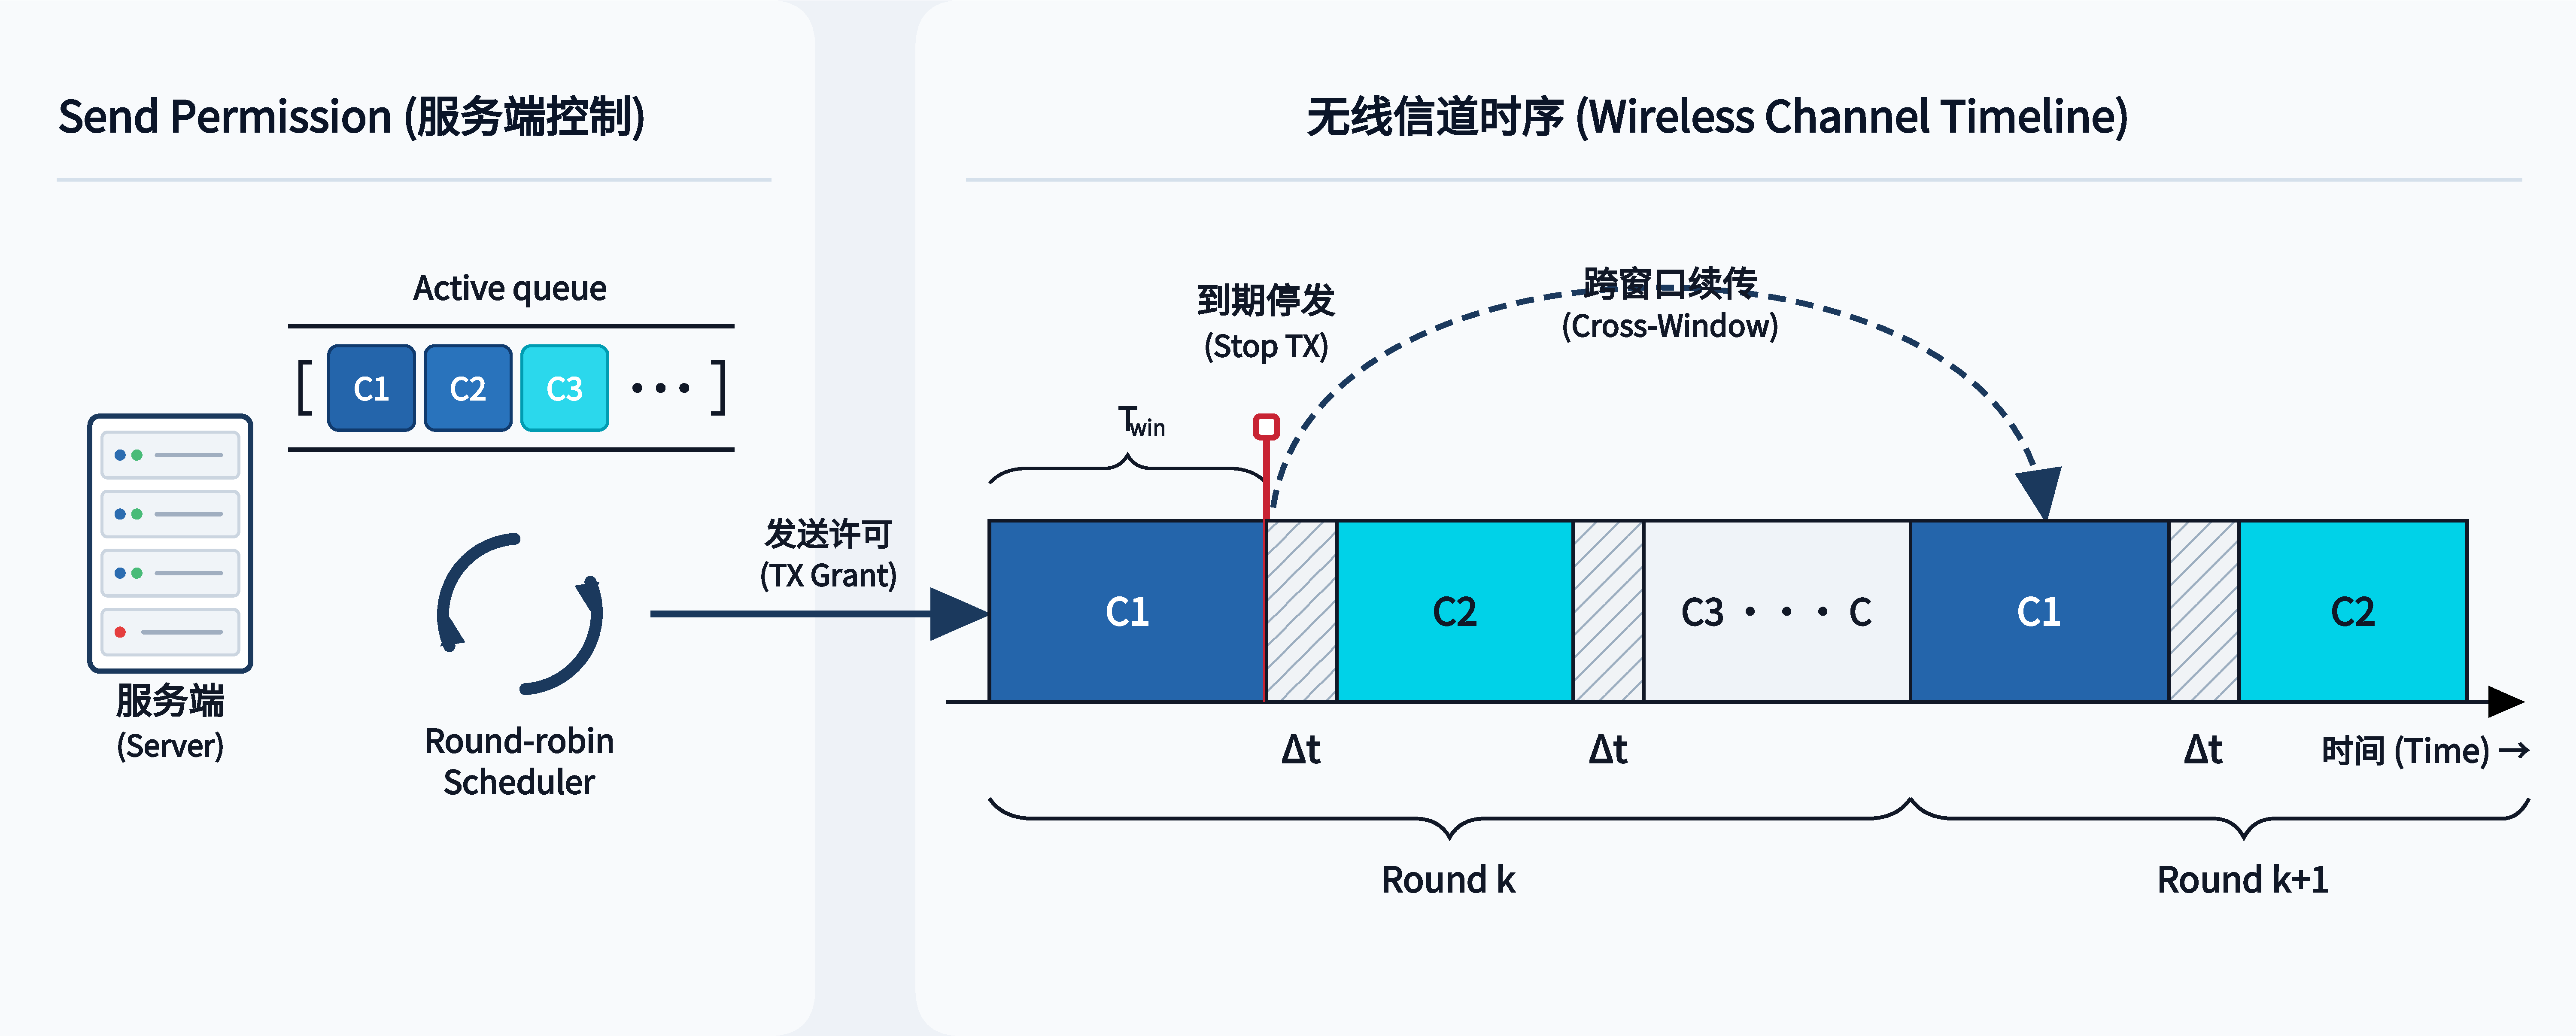
\includegraphics[width=\textwidth]{figure2.pdf}
\caption{发送权轮转与限时发送窗口。}
\label{fig:2}
\end{figure*}

下行阶段的结束包含客户端与服务端两个层次的完成判定。任何一个客户端在本地通过 UFTP 接收到完整模型文件，并通过运行层的格式与 SHA-256 摘要校验后，即可立即返回模型路径并启动本地训练，不必等待其他客户端同步完成。服务端的运行层则必须等待传输适配层确认全部预期目标客户端均已可靠收到模型文件，方才越过下行完成屏障。下行完成屏障只约束服务端的模型发布判定，为全局轮次立下交付基线；只要本地校验通过，客户端尽可直接进入训练，不必受其约束。

客户端完成本地模型训练后，生成各自的更新文件并进入更新回传阶段。各客户端本地训练产生的数据更新各不相同，属于典型的多对一独立文件提交，上行传输因而选择 HTTP PUT 配合底层 TCP 协议。HTTP PUT 提供了成熟的请求响应语义、内容长度界定与状态码规范；底层的 TCP 协议则保证了字节流可靠有序。平台在传输适配层中额外执行客户端身份核验、文件长度比对与数据摘要验证，确保更新文件的完整性，不把全部校验责任推给 HTTP 协议本身。客户端更新数据进入链路控制层的发送队列后，队列由空变为非空触发客户端向上发送就绪声明。服务端完成合法性校验后将客户端加入活跃队列，并复用下行建立的发送权轮转机制（如 Fig.~\ref{fig:2} 所示），按顺序轮流为客户端授予限时发送窗口。上行传输同样依靠链路层前向纠错抵御无线丢包，剩余的字节流缺失则由 TCP 的确认与重传机制处理。在各客户端的普通上行发送机会之间，服务端保留短暂的反向传输机会以回传 TCP 确认帧，保证双向流控正常推进，该反向机会不同于下行 UFTP 的周期性反馈轮。

客户端模型更新文件体积通常达到数十兆字节，远超单个发送窗口所能承载的容量，必须跨越多个限时发送窗口持续推进。单次窗口到期只是暂停网卡的无线发送。传输适配层已经建立的 HTTP 连接依然维持，未发完的请求也不会撤回；待发数据留在本地发送队列中，等下一个许可窗口打开，接着往前传，不用重建连接，更不用重发数据。仅当发生网络超时或物理连接断开时，系统才按传输契约判定失败，并不承诺任何异常下连接绝对不中断。

链路控制层维护固定容量的用户态出站发送队列，承接已从 TUN 读取但尚未发出的数据面流量。为防止数据源源不断注入导致队列无限膨胀乃至内存耗尽，系统设置高低两道字节积压水位以及数据包数量硬上限。当队列中积压的待发字节达到高水位阈值时，链路控制层主动暂停从 TUN 虚拟网卡读取新数据，通过系统网络栈自身的流控机制向上层应用形成反压。当积压数据随空口发送减少、降至低水位阈值后，系统重新恢复从 TUN 读入。双阈值构成的滞回区间可有效避免临界点上的频繁启闭（见 Fig.~\ref{fig:3}）。数据包数量硬上限独立发挥作用，防止大量小尺寸数据包在未触碰字节水位前耗尽队列索引。相同的队列容量约束、双水位滞回与反压机制，同样适用于服务端的下行数据发送。此处起伏变化的是随传输节奏波动的队列积压量，阈值本身属于静态预设参数，并不存在随链路状态自动调整的复杂算法。

% 原稿标记保留：**[Figure 3 占位 队列水位与反压机制图]**

% 原稿题注保留：> Figure 3 解释出站发送队列的字节积压变化，以及达到高水位暂停从 TUN 读入、降至低水位恢复读入的反馈调节关系。

\begin{figure*}[t]
\centering
% 裁去图稿上下的纯白外边距，保留所有图内元素；PDF 文件本身不变。
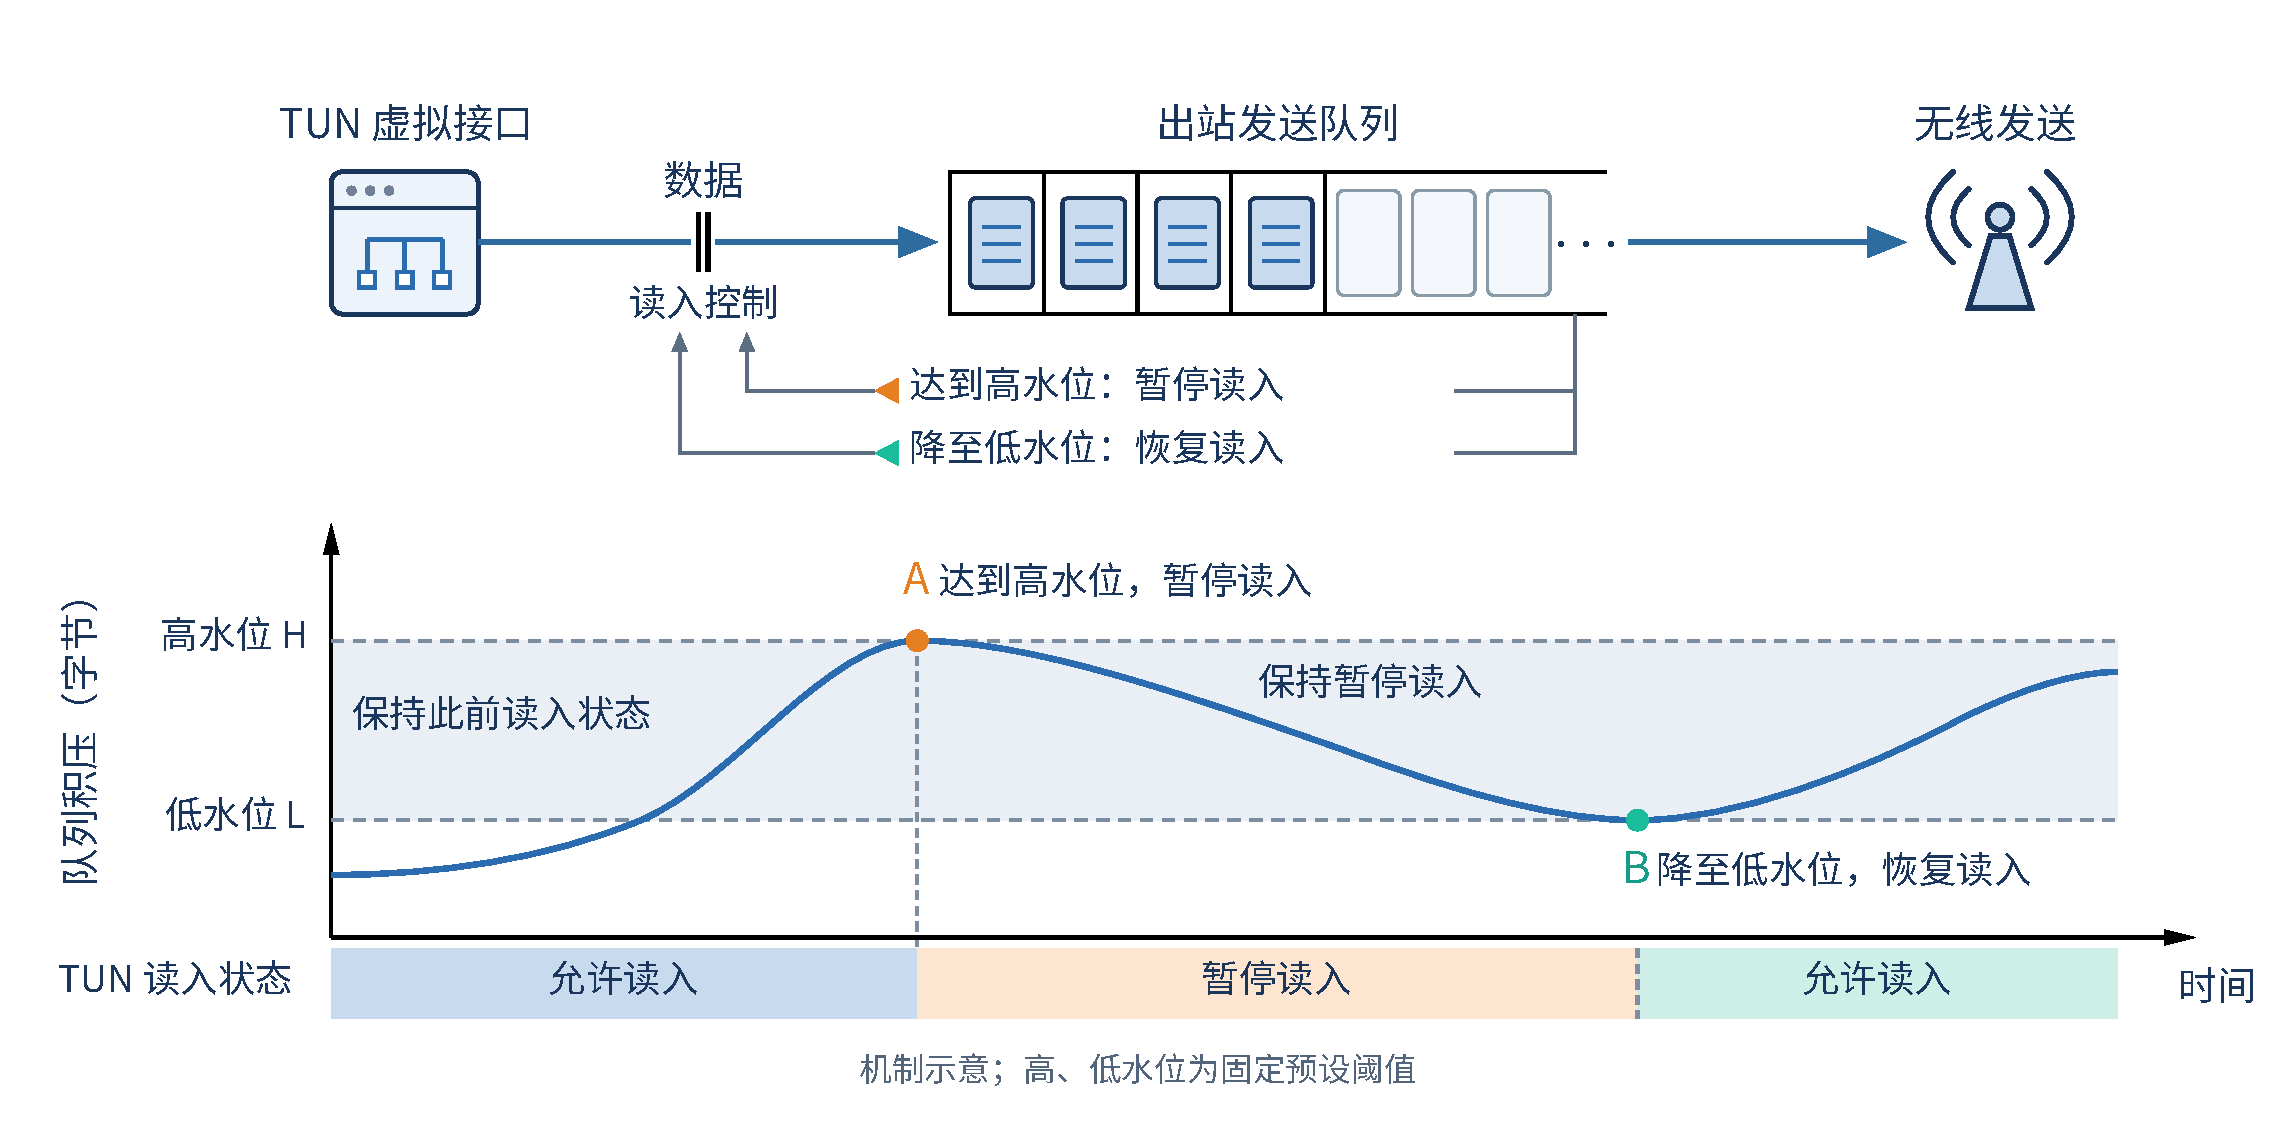
\includegraphics[width=\textwidth,trim=0 2bp 0 32bp,clip]{figure3.pdf}
\caption{出站发送队列的双水位反压机制。}
\label{fig:3}
\end{figure*}

就绪声明与发送许可等链路调度控制消息走独立的优先通道，直接经由无线收发层收发，不进入出站发送队列，也不经过 TUN 接口。即使普通数据队列处于高水位积压或处于反压停读状态，调度控制帧依然可以顺畅收发，避免大文件传输阻断调度控制。出站发送队列与入站接收重组缓冲在职责上保持独立。出站队列承接本机向外发送的数据，入站接收重组缓冲则承接从无线信道接收的数据分片，负责处理乱序到达、分组缺片以及前向纠错恢复。多个客户端交替上行时，服务端接收端根据每个无线分片中携带的发送者身份标识，对不同客户端的数据块分别进行隔离重组，防止多节点数据混合错乱。接收重组缓冲的积压或淘汰同样独立于控制通道，不能影响调度控制消息的正常收发。

一轮训练的最终收束涉及多层完成判定的协同，各层边界不可相互替代。发送许可生效仅代表客户端取得了在无线信道上的发送机会。服务端 monitor 模式捕获到无线帧仅证明物理信号到达本机，不等于上层接收到合法文件。单个客户端的更新文件在传输适配层通过长度比对与 SHA-256 摘要核验，并在服务端存储路径完成原子文件提交后，才构成该客户端更新文件的正式提交。服务端运行层在确认下行完成屏障已经达成、且本轮预期的全部有效客户端更新文件均已完整收齐后，才将全部更新文件打包交付联邦学习算法层执行全局模型聚合。单个客户端提交成功绝不等于整轮联邦学习成功，只有全部有效更新完整入库才能驱动算法层完成本轮训练。

\section{真实硬件实验与结果评估}
\label{sec:4}

前文交代了 WFB-FL 怎样在原始无线帧路径上组织收发协同与调度。进入物理实验，我们关注两件事。一是这六项无线参数在真实硬件上能支持到什么范围，二是在学习任务、节点规模与计算条件保持一致时，不同的无线配置怎样改变多客户端训练的通信表现与整轮耗时。为此，我们在由真实边缘计算节点与消费级 802.11 无线网卡搭建的物理测试台上开展实验评估。

\subsection{实验设置}

真实硬件实验平台由 1 台参数服务端与 10 台边缘客户端组成，节点计算设备采用 Jetson Orin Nano 边缘计算板卡，各节点均外接消费级 RTL8812AU 双频 USB 无线网卡，驱动采用开源的 rtl88xxau\_wfb 实现。全部节点部署于面积约 120 平方米的典型室内办公环境中，各客户端分散放置在不同工位与隔断间，节点间距在 3 至 12 米之间，包含直射视距与穿透隔断的非视距反射路径，构成典型的室内多径与阴影衰落效应。无线信道处于包含邻近商用 Wi-Fi 弱干扰的真实室内电磁环境。在联邦学习工作负载方面，实验采用 ResNet-18 深度神经网络模型与 CIFAR-10 图像分类数据集构建同步联邦学习任务，单次模型广播分发的数据文件大小固定为 40 MiB（约 41.9 MB）。整个实验过程基于真实物理硬件、真实操作系统网络栈与真实无线链路收发闭环运行，不采用网络仿真器或单机多进程模拟。

\subsection{可配置无线参数}

在此硬件平台上，WFB-FL 支持对工作信道、信道带宽、调制编码方案（MCS）、保护间隔（GI）、前向纠错（FEC）冗余以及发射功率六项关键无线参数实施显式配置。六项参数平级列出，各自对应物理层收发与链路控制层不同的调控维度，共同为构建不同的无线工作条件提供参数依据。Table~\ref{tab:2} 汇总了当前硬件环境下各项无线参数的可配置取值与硬件支持范围。

% 原稿标记保留：**[Table 2 占位 六项无线参数的可配置取值与硬件支持范围]**

% 原稿题注保留：> Table 2 平级列出信道、带宽、MCS、保护间隔、前向纠错和发射功率的可配置取值与硬件支持范围，为三种无线配置提供依据。

\begin{table*}[tb]
\caption{六项无线参数的可配置取值与硬件支持范围。}
\label{tab:2}
\centering
\small
\renewcommand{\arraystretch}{1.25}
\setlength{\tabcolsep}{5pt}
\begin{tabularx}{\textwidth}{@{}>{\raggedright\arraybackslash}p{0.15\textwidth}YY@{}}
\toprule
\textbf{无线参数类别} & \textbf{典型可配置取值范围} & \textbf{硬件与系统支持范围及约束} \\
\midrule
\textbf{工作信道} & 2.4 GHz（Ch 1 至 13）与 5 GHz 频段主流信道（如 5 GHz Ch 157） & 取决于 RTL8812AU 射频芯片支持范围及所在地区无线电管理频谱法规 \\
\textbf{信道带宽} & 20 MHz 与 40 MHz（HT20 / HT40+） & 取决于网卡射频基带芯片与驱动对频宽切换的支持能力 \\
\textbf{调制编码（MCS）} & MCS 0 至 MCS 7（802.11n 单天线单流调制编码，BPSK 至 64-QAM） & 取决于射频基带支持的调制阶数与编码率 \\
\textbf{保护间隔（GI）} & 长保护间隔（Long GI, 800 ns）与短保护间隔（Short GI, 400 ns） & 取决于基带芯片符号时序控制与驱动对短保护间隔特性的支持 \\
\textbf{前向纠错（FEC）} & Cauchy-Reed-Solomon 纠错码冗余（RS(8, 10) 至 RS(8, 14) 块级冗余配置） & 由链路控制层软件实现，受边缘节点 CPU 编解码计算负载约束 \\
\textbf{发射功率} & 10 dBm 至 20 dBm（综合实验固定为 17 dBm） & 受 RTL8812AU 射频功放物理上限及 Linux 内核无线驱动接口支持范围约束 \\
\bottomrule
\end{tabularx}
\end{table*}

\subsection{完整 FL 综合实验}

为评估物理无线条件对联邦学习端到端训练的影响，我们设计并执行了多客户端联邦学习综合实验。该实验回答一个核心问题。当模型架构、训练数据集、参与节点规模、本地计算步数、工作信道（固定为 5 GHz Ch 157）、发射功率（固定为 17 dBm）以及空间物理拓扑保持一致时，不同的预设无线配置怎样改变多客户端联邦学习的通信表现与整体轮次耗时。

依据 Table~\ref{tab:2} 所列的硬件支持范围，实验预设了三种典型无线配置，分别命名为稳健性优先、折中以及吞吐优先。配置命名仅代表预先设定的参数设计取向，具体参数组合在正式实验数据采集前固定，三组配置全部无偏地进入端到端综合实验，不根据后验测试表现对配置进行反向筛选。稳健性优先配置采用 20 MHz 信道带宽、MCS 2（QPSK 3/4）、长保护间隔与 RS(8, 14) 纠错冗余（约 42.8\% 冗余），旨在恶劣信道下优先保证低误码与确定性；折中配置采用 20 MHz 信道带宽、MCS 4（16-QAM 3/4）、短保护间隔与 RS(8, 12) 纠错冗余（33.3\% 冗余），在基础速率与抗扰度间寻求平衡；吞吐优先配置采用 40 MHz 信道带宽、MCS 6（64-QAM 3/4）、短保护间隔与 RS(8, 10) 纠错冗余（20.0\% 冗余），旨在最大化瞬时物理发射速率。

在综合实验执行与统计口径上，每种配置均独立执行 10 次完整的多客户端联邦学习训练，每次训练包含 5 轮严格闭环训练，同一次训练中的各轮次仅反映训练时序推进，不作为独立重复样本。综合实验对全部尝试的完成情况进行完整记录与如实呈现，不静默删除任何失败或超时的运行。核心评价指标包括模型下行有效吞吐、客户端更新提交情况与完整轮次耗时三项。模型下行有效吞吐定义为单次广播的模型文件总大小除以全体目标客户端均成功完成完整模型文件接收与校验所需的总交付时间；客户端更新提交情况记录各客户端在限时发送窗口轮转调度下的轮内实际提交时刻与提交成功状态；完整轮次耗时严格从服务端发布该轮模型开始计时，历经下行可靠广播、各客户端本地计算以及多客户端轮转上行提交，直至服务端收齐本轮预期有效更新并完成算法聚合时为止。客户端在本地校验模型后即可立即训练（单节点单轮计算耗时约 10 至 12 秒），部分较快完成计算的客户端会在其他客户端仍在计算时提前提交更新，下行交付、本地训练与上行回传在时间上形成流水线重叠，各阶段耗时不能简单相加。

% 原稿标记保留：**[Figure 4 占位 综合实验结果组合图]**

% 原稿题注保留：> Figure 4 展示三种预设无线配置下的模型下行有效吞吐、客户端更新提交情况和完整轮次耗时，交代全部尝试的完成情况。

\begin{figure*}[tb]
\centering
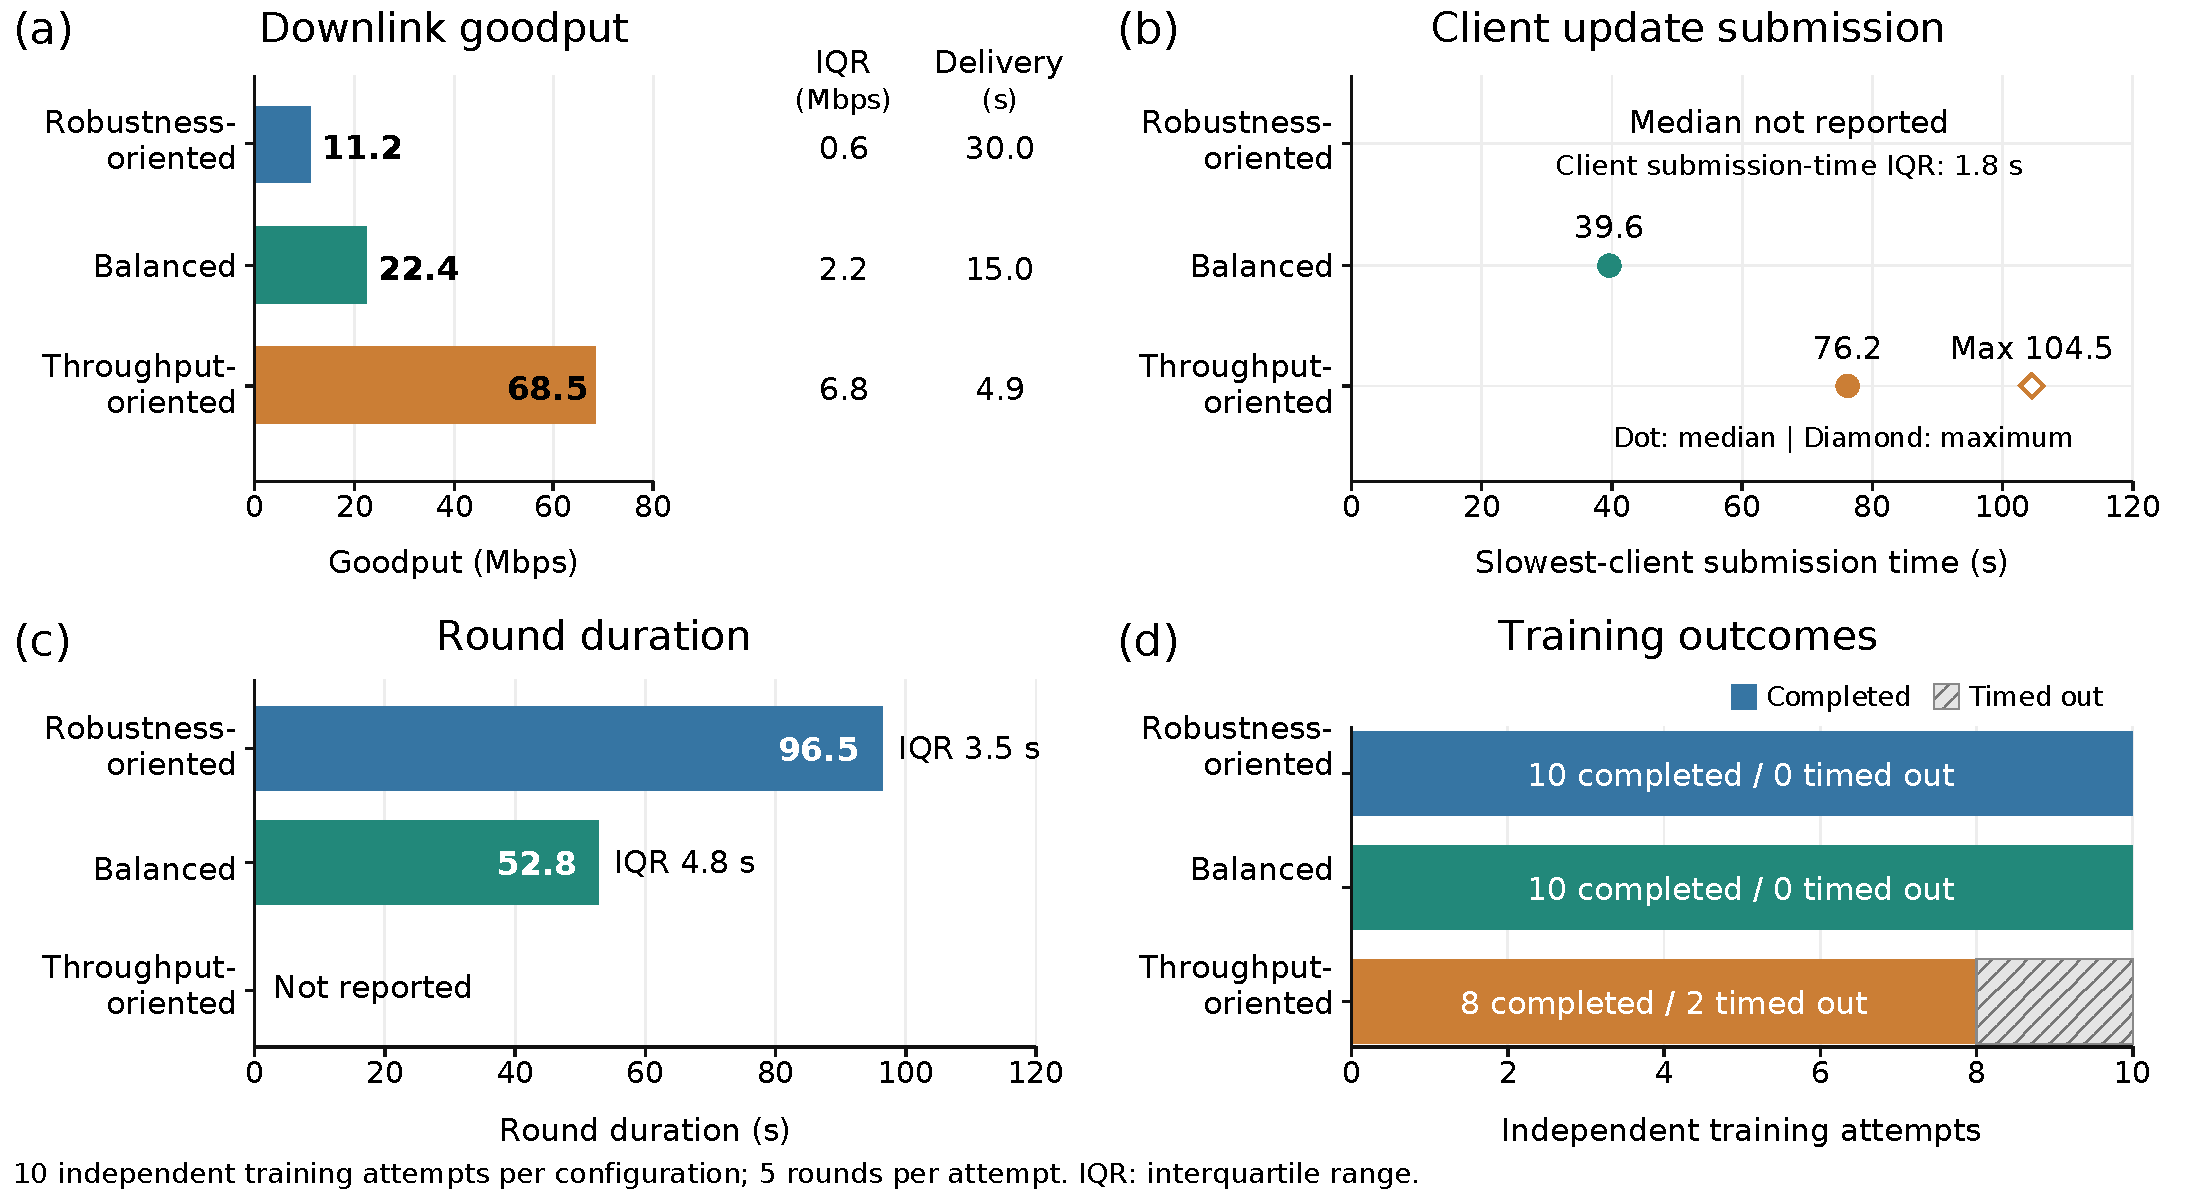
\includegraphics[width=\textwidth]{figure4.pdf}
\caption{三种预设无线配置的综合实验结果：（a）下行有效吞吐；（b）客户端更新提交；（c）完整轮次耗时；（d）训练尝试的完成情况。每种配置独立尝试 10 次训练，每次 5 轮；IQR 表示四分位距。}
\label{fig:4}
\end{figure*}

Figure~\ref{fig:4} 综合展示了三种预设无线配置在多次独立训练中的测量结果分布。定量比较表明，不同的无线参数组合对联邦学习端到端轮次呈现出显著不同的系统影响。在模型下行分发阶段，吞吐优先配置依托高阶调制与较高带宽，下行有效吞吐达到 68.5 Mbps（四分位距 6.8 Mbps），交付耗时仅为 4.9 秒；但在上行更新阶段，高阶调制在实际空间多径扰动下容易丢包，导致部分弱信号客户端在轮转调度中经历更多重传，最慢客户端的提交耗时呈现严重长尾拖尾，中位数达到 76.2 秒（极值达 104.5 秒）；相比之下，稳健性优先配置在下行阶段的有效吞吐为 11.2 Mbps（四分位距 0.6 Mbps），分发耗时为 30.0 秒，但各客户端提交时刻表现出高度集中的一致性（四分位距仅 1.8 秒，无长尾拖尾），整轮耗时分布在中位数 96.5 秒（四分位距 3.5 秒）；折中配置的下行有效吞吐达到 22.4 Mbps（四分位距 2.2 Mbps，分发耗时 15.0 秒），各客户端提交平稳推进（最慢客户端耗时中位数 39.6 秒），整轮耗时中位数为 52.8 秒（四分位距 4.8 秒）。在全部 10 次独立训练尝试中，稳健性优先配置成功闭环 10 次（10 次成功，0 次超时），折中配置成功闭环 10 次（10 次成功，0 次超时），吞吐优先配置成功闭环 8 次，其余 2 次因隔断弱信号节点上行停滞超时未完成（8 次成功，2 次超时失败）。

上述测量结果表明，在相同的算法与计算负载下，底层物理无线条件直接改变模型分发与更新提交的时间分配，名义物理速率最高并不保证整轮训练耗时最短。这一系统含义进一步印证了将无线链路转变为显式可控实验对象的必要性。同时，本实验的证据边界严格立足于固定拓扑、特定硬件与上述预设配置组合的整体表现，结果差异归因于整套无线配置在特定物理环境中的综合效果，不孤立归因于某一单项物理参数，不将配置映射为外部设备类型，亦不据此声称该组合在算法收敛精度上带来改善或优于商用黑盒 Wi-Fi 协议栈。

\section{讨论与后续研究}
\label{sec:5}

本文平台面向分布式算法、计算负载与节点拓扑相对固定的测试场景，支持主动设置一组无线收发参数，进而定量比较端到端训练轮次的通信开销。受控比较能够成立，依赖底层配置的确定性，以及通信对端对帧级元数据的准确记录。这就对硬件提出了明确要求。实验能力的实际覆盖面，主要受制于所选网卡、射频芯片以及系统驱动的开放程度。不同硬件对频宽切换、调制编码等级以及元数据暴露的支持各不相同，部分消费级网卡驱动并未开放全部底层读写接口。测试环境同样划定了适用边界。在特定室内测得的传输表现与耗时分布，深受房间格局、天线摆放以及背景电磁干扰影响，相关结论无法直接外推至室外远距离传输、高速移动或强干扰等工业车载环境。清楚这些使用条件，才能在合理的边界内展开有针对性的实验设计。

当协同训练的客户端从十余台继续增加时，通信组织的效率权衡开始发生变化。在下行阶段，一对多广播展现出极高的复用价值。无论接收节点增加多少，模型文件在空中只需广播一次，通信负载不会随设备数量成倍增加。上行阶段则完全不同。每个客户端必须独立提交各自计算得到的更新文件。现有平台依托模型广播分发、限时发送权轮转与聚合屏障，保证了多节点交替上传时不会互相冲撞。然而，排队等待许可的节点一旦增多，调度轮询的切换间隙、传输过程中的反向确认，以及慢速节点带来的同步拖尾，都会增加整轮训练的时间负担。下行广播节省的时间能否抵消轮转调度与长尾等待的开销？这一得失平衡在更大规模的网络中究竟如何演变，需要进一步的实证测量。如何在多节点集群中更灵活地协调发送机会与反馈窗口，进而保持整轮协作的高效推进，构成了后续优化通信组织的核心问题。

当训练任务发生变化时，模型体积可能从数兆字节延伸至数百兆字节，本地计算耗时也从数秒跨越到数分钟，各个客户端所处的信道质量更往往参差不齐。在如此差异化的场景下，单一的无线配置很难在整轮训练中始终保持全局高效。显式参数配置与全流程比较提供了观察手段，但不同配置在上下行阶段的收益权衡大相径庭。追求高速率的配置能迅速完成下行模型广播，可一旦遇到信道衰落严重的弱链路节点，上行回传容易出现大量丢包与重传，拖垮整轮进度。低阶调制配合高冗余纠错能够稳妥应对恶劣链路，却又会在下行阶段消耗过多时间。如何在模型规模、计算耗时与链路质量各不相同的情况下确定合理的无线配置，需要更系统的方法支撑。推进这一课题，不仅要在多种神经网络结构与复杂的物理传播环境中展开广泛验证，也需要结合具备更高吞吐特性的新一代无线网卡设备开展长期的对比测试。


\end{document}
